\section{Implementation} \label{sec:Implementation}
Vor der Implementation ist die Entscheidung der Auswahl der Einzelkomponenten, welche im Abschnitt \ref{Architektur} vorgestellt wurden, zu treffen.
\\ \\
Zuerst ist die Programmiersprache sowie das genutzte Framework zu definieren.
Aus Erfahrungsgründen wurde das C\# Framework ASP.NET gewählt.
Mit diesem lassen sich unter anderem API-Services bauen.
ASP.NET hat mit Visual Studio auch direkt eine Entwicklungsumgebung sowie Debugging Möglichkeiten.
Weiterhin gibt es die Möglichkeit die eingebette NoSQL-Datenbak LiteDB zu nutzen.
Durch die große und aktive Community von ASP.NET ist dieses Framework sehr gut dokumentiert und es existieren viele Open-Source-Bibliotheken.
\subsection{Experimente} \label{sec:Experimente}
    Aus der Forschungsfrage \ref{q:five} ergeben sich Experimente, die auf Skalierbarkeit und Laufzeit der API abziehlen.
    \subsubsection{LiteDB Pipeline} \label{sec:ExperimentePIPE}
    Um die Suche von mehreren Paketen in der Datenbasis zu beschleunigen wurde sich das Prinzip der Parallelisierung zu Nutzen gemacht.
    Hierzu wurde die zu untersuchende Liste von Paketen auf verschiedene Tasks aufgeteilt.
    So ist nach dem vollständigen Befüllen der Pipeline eine theoretischen Laufzeitverkürzung um der Faktor der maximal abarbeitbaren Tasks erreicht.  
    
    Dabei sind zwei Fälle zu unterscheiden:
    \begin{description}
        \item[\textit{Weniger} Pakete als Datenbank-Dateien]\hfill \\
            In diesem Falle einer geringeren Anzahl an Pakete wird die Pipe nie vollständig gefüllt.
        \item[\textit{Mehr} Pakete als Datenbank-Dateien]\hfill \\
            In jenem Falle muss die Paketliste Stück für Stück in die Pipe eingefügt werden und beim Erreichen der Kapazität -- entsprechend der Anzahl der Datenbanken -- das früheste Paket entfernt und ein neues Paket am Anfang eingefügt werden.
    \end{description}
    
    Die Verwaltung der 3 verschiedenen Staaten der Pipe ist in folgender Abbildung mit \ac{PAP} nachvollziehbar.
    Anschließend sind die 3 Fälle näher ausgeführt.
    \begin{figure}[H]
        \centering
        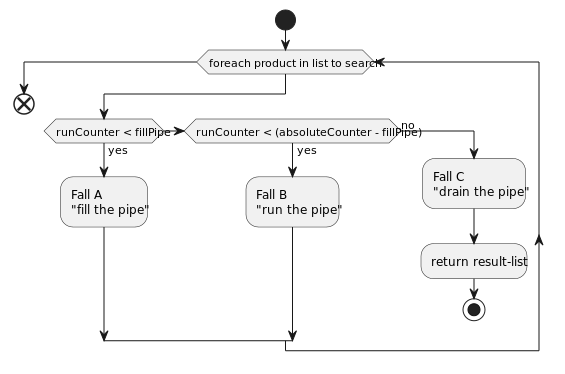
\includegraphics[width=\textwidth]{../pap/Simultanius search on LiteDb-Files.png}
        \caption{Übersicht der Pipeline-Staaten}
        \label{png:OverviewPipelineStatus}
    \end{figure}

    Das Befüllen der Pipeline geschieht nach folgendem Muster:
    \begin{figure}[H]
        \centering
        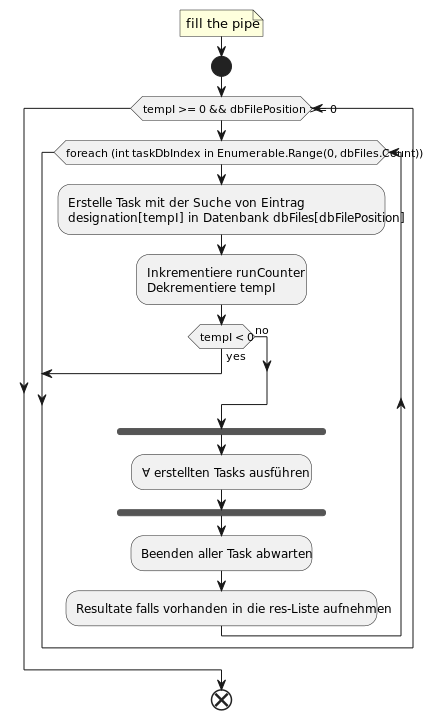
\includegraphics[width=\textwidth]{../pap/Case_A.png}
        \caption{\ac{PAP} Befüllen der Pipeline}
        \label{png:case_a}
    \end{figure}

    Nach vollständiger Befüllung die Erhaltung der Pipeline:
    \begin{figure}[H]
        \centering
        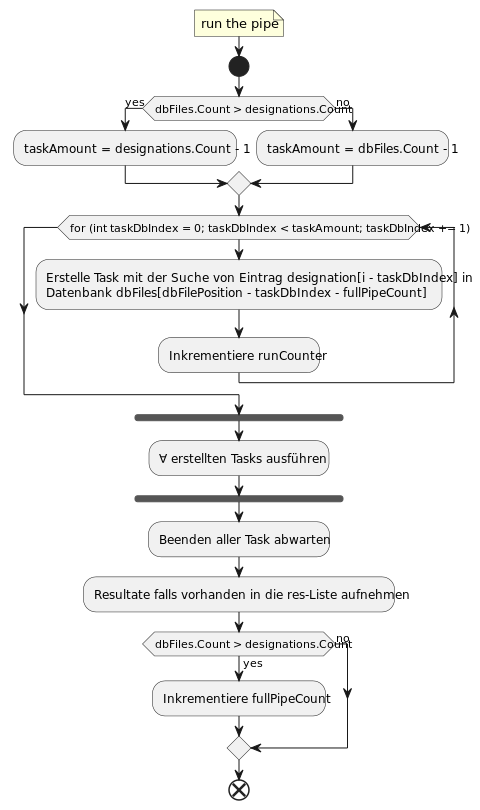
\includegraphics[width=\textwidth]{../pap/Case_B.png}
        \caption{\ac{PAP} Aufrechterhalten der Pipeline}
        \label{png:case_b}
    \end{figure}

    Beim Leeren der Pipeline:
    \begin{figure}[H]
        \centering
        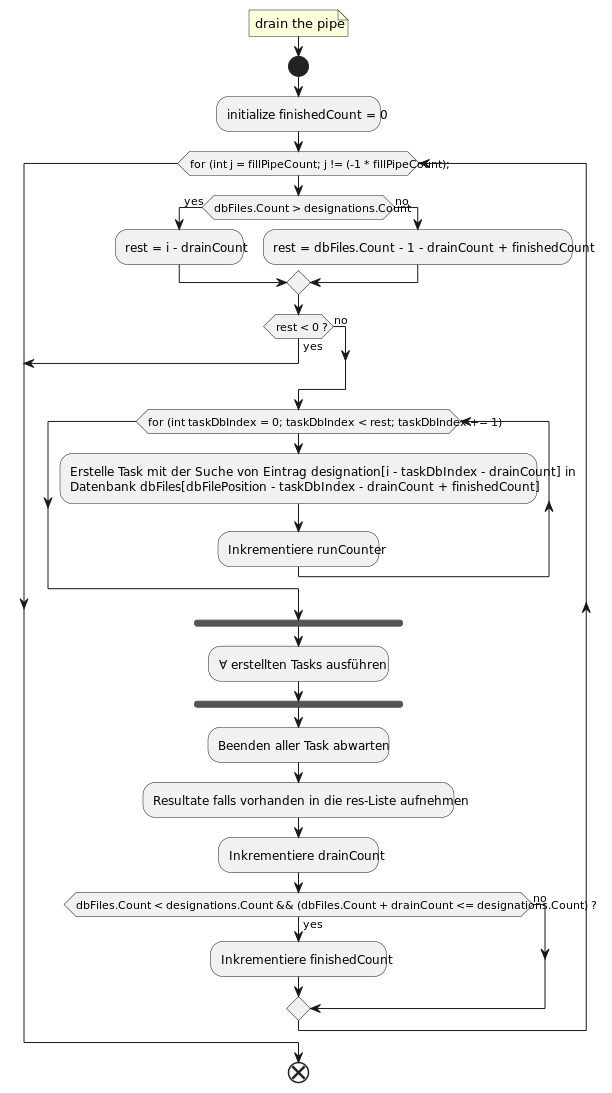
\includegraphics[width=\textwidth]{../pap/Case_C.png}
        \caption{\ac{PAP} Leeren der Pipeline}
        \label{png:case_c}
    \end{figure}

    Aus der Implementation der Pipeline ergeben sich folgende Laufzeiten bei weniger Paketen als Datenbankdateien:
    \begin{tabular}{|c|c|c|}
        \hline
            Such-Typ & Zeit & Faktor \\
            Mono-Suche & 262676.7ms & 1 \\
            Pipeline & 96868.4ms & 2.7213448 \\
        \hline
    \end{tabular}

    Aus der Implementation der Pipeline ergeben sich folgende Laufzeiten bei weniger Paketen als Datenbankdateien:
    \begin{tabular}{|c|c|c|}
        \hline
            Such-Typ & Zeit & Faktor \\
            Mono-Suche & 95011.24ms & 1 \\
            Pipeline & 22111.5ms & 4.296846569 \\
        \hline
    \end{tabular}

    \subsubsection{Datenbank} \label{sec:Experimente}
Die Wahl der Datenbank hat einen großen Einfluss auf die Laufzeit von Anfragen auf diese.
Aus der Gegebenen Einbindung einer NoSQL Datenbanklösung in ASP.NET, LiteDB, wurde diese auch zuerst als Datenspeicher gewählt.
\\
--> reicht diese Begründung für die Entscheidung? \\

Wieso Entscheidung auf Änderung? \\

Vergleich Messwerte (Am besten Messreihen) in Tabelle auf welchen Datenmengen? \\

--> Entscheidung auf welche DB am Ende, weil? \\
--> Einsparung von was am Ende? \\
    \subsubsection{MySQL Indexierung} \label{sec:MySQL_Indexierung}
    Die expliziten gemessenen Differenzen zwischen der Suche auf einer und der selben Tabelle einmal mit und einmal ohne erzeugten Index kann im Appendix unter \ref{subsec:MySQLMitIndex} \& \ref{subsec:MySQLOhneIndex} eingesehen werden.
    \\
    Eine Indizierung auf einer Tabelle in MySQL erzeugt Bereiche auf der Spalte, mit denen die Suche sehr beschleunigt werden.
    Laut der offiziellen Webseite von MySQL ist ohne Index die Suche auf einer Tabelle sequenziell von oben nach unten.\textsuperscript{\cite{link:MySqlIndex}}
    Dagegen ermöglicht die Suche mit einem erstellten Index der Datenbank, schon beim ersten Tabellenzugriff lediglich einen Bereich von Datensätzen zu durchsuchen.
    Damit sollte die Leistung merklich verbessert werden.
    \\
    Nachfolgend die arithmetische Mittel aus jeweils 10 Messungen auf der selben Tabelle mit und ohne Index:
    \\
    \begin{tabularx}{0.8\textwidth}{|c|c|c|}
        \hline
        Such-Typ & Zeit & Faktor \\ \hline
        ohne Index & 207,86ms & 1 \\
        mit Index & 0,710666667ms & 292,48593 \\
        \hline
        \caption{Laufzeiten Durchschnitt 10 Messungen \textsuperscript{siehe Appendix \ref{subsec:MySQLMitIndex} \& \ref{subsec:MySQLOhneIndex}}}
        \label{tabularx:MySqlIndexWithAndWithout}
    \end{tabularx}

    %!!!! SUCHE AUF JSON VS DB FILE
    Experimente
    \begin{itemize}
        \item Laufzeitmessungen LiteDB (Mono vs. Pipe -- schon schneller, aber nicht genug $\rightarrow$ fragments/searchStatistics.md)
        \item conclusio geht es schneller mit einer relationalen Datenbank?
    \end{itemize}